\chapter{Attitude Controller Test Setup}\label{app:AttitudeControllerTest} 
This appendix describes the equipment needed and the considerations needed when using the set up utilized to test he attitude controller on the quadcopter.
\subsubsection{List of Equipment}
\begin{table}[H]
	\centering
	\begin{tabular}{|c|c|}
		\hline%------------------------------------------------------------------------------------------------------------
		\textbf{Instrument}   &  \textbf{AAU-no.}  \\
		\hline%--------------------------------------\\----------------------------------------------------------------------
		Quadcopter    	&  - 					  \\
		\hline%------------------------------------------------------------------------------------------------------------
		Vicon System 			& 75459             \\   
		\hline%------------------------------------------------------------------------------------------------------------
		Computer with MATLAB       &  A6703		\\
		\hline%------------------------------------------------------------------------------------------------------------
		Attitude quadcopter holder      &  -		\\
		\hline%------------------------------------------------------------------------------------------------------------
		Attitude quadcopter connector    &  -	\\
		\hline%------------------------------------------------------------------------------------------------------------
	\end{tabular}
\end{table}
\subsubsection{Setup}

\autoref{fig:AttitudeControllerTestsetup} shows the test set up used when testing the attitude controller.

\begin{figure}[H]
	\centering
	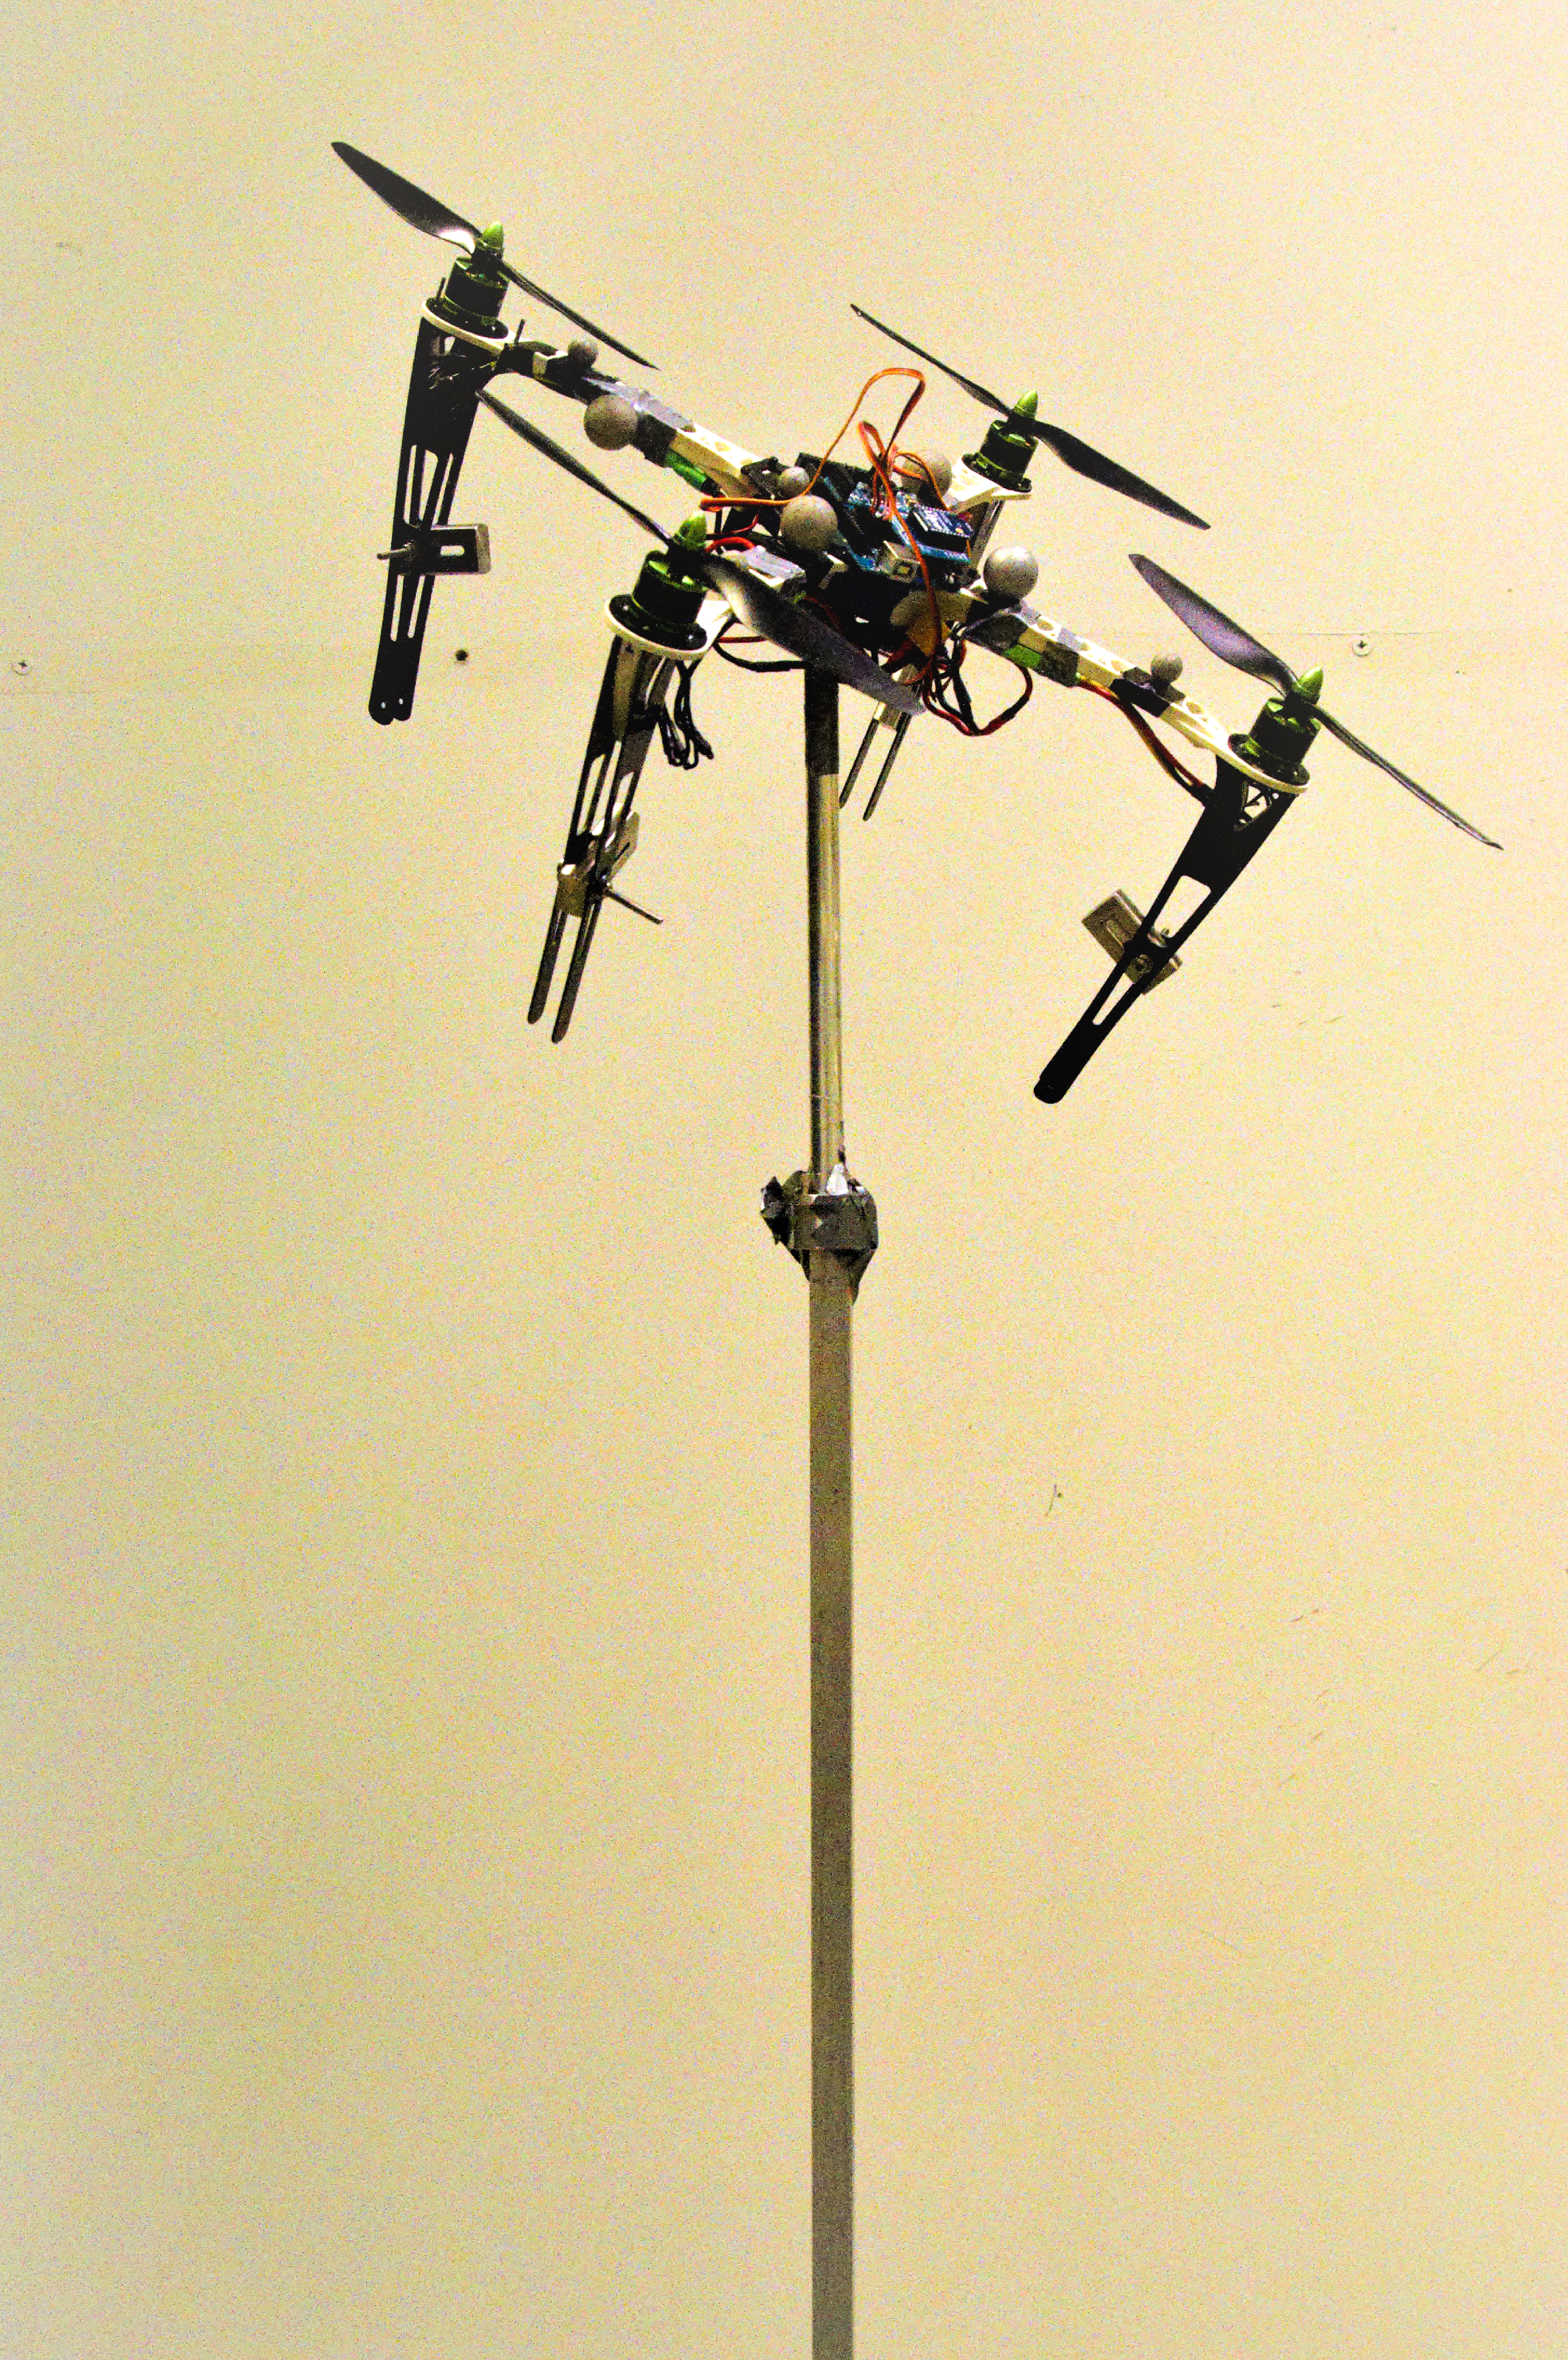
\includegraphics[scale=0.1]{figures/AttitudeSetUp}
	\caption{The test setup utilized to test the attitude controller.}
	\label{fig:AttitudeControllerTestsetup}
\end{figure}

The set up distorts the moments of inertia around the different axes and the location of the center of rotation with respect to the center of mass. The latter is especially critical as the quadcopter behaves like an inverted pendulum. To counteract this effect, the center of mass of the quadcopter must be moved down. This is done placing masses in the four arms of the quadcopter and below the center of rotation. 

